\clearpage
\subsection{Program (with Procedures)} % (fold)
\label{sub:program_with_procedures_}

Each Program is a list of instructions (\nameref{sub:statement}s) that command the computer to perform actions. Unfortunately the computer is only able to perform simple actions, meaning that even small programs need many instructions in order to perform their tasks. To help manage these instructions you can group the program's Statements into Procedures, creating Procedures that perform the tasks you need completed in your Program.

\begin{figure}[h]
   \centering
   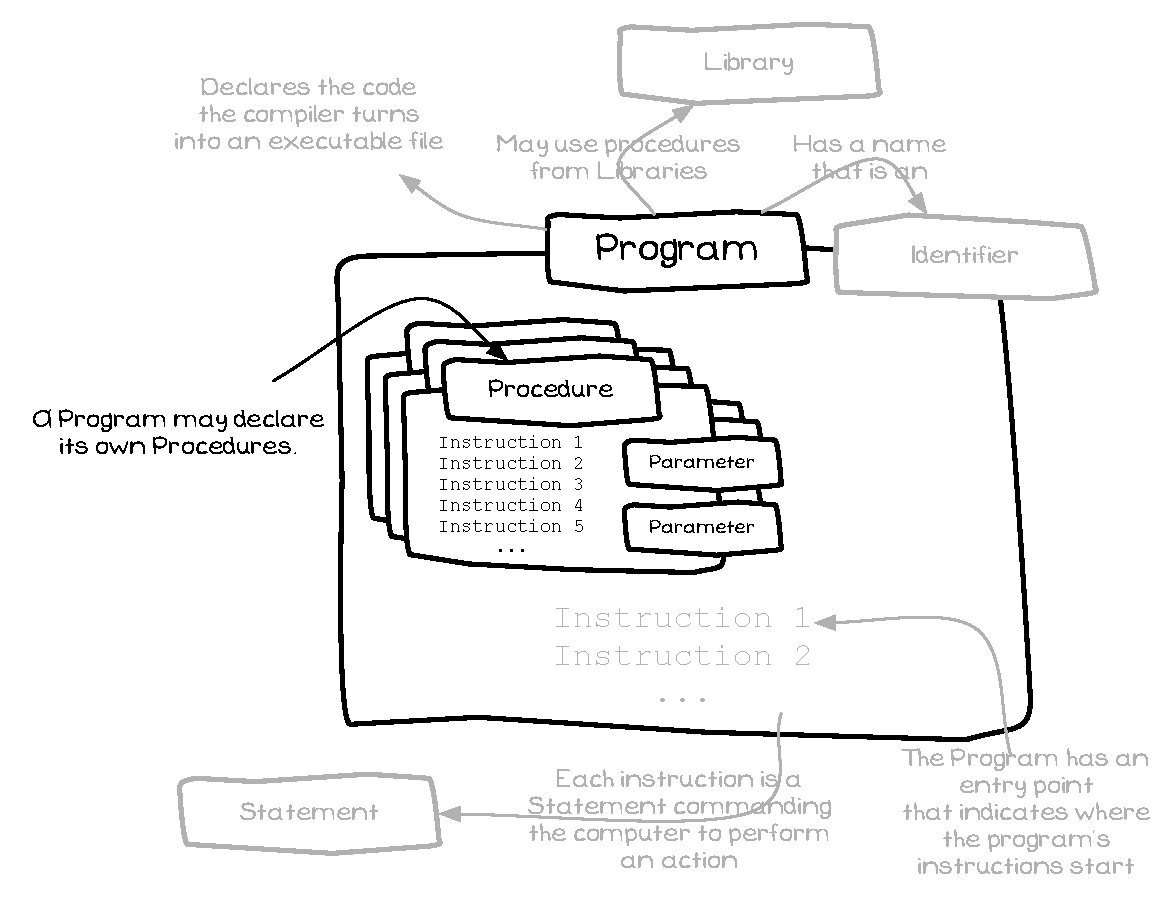
\includegraphics[width=\textwidth]{./topics/program-creation/diagrams/ProgramWithProc} 
   \caption{Program with Procedures}
   \label{fig:procedure-decl-program}
\end{figure}

\mynote{
\begin{itemize}
  \item A Program is an \textbf{artefact} that you can \emph{create} in your code.
  \item A Program can contain a number of \nameref{sub:procedure}s.
  \item \nameref{sub:proc_decl-procedure_declarations} allow you to create your own Procedures.
  \item The program's instructions can call the Procedures you create in the program's code.
  \item In C and Pascal the \nameref{sub:proc_decl-procedure_declarations} must appear before they are used in your code.
\end{itemize}
}

% subsection program_with_procedures_ (end)